% % % % % % % % % % % % % % % % % %
%                                 %
%  Master Thesis                  %
%  MSc in Aerospace Engineering   %
%  Mattia Gregnanin               %
%  A.Y. 2025/2026                 %
%                                 %
% % % % % % % % % % % % % % % % % %
%                                 %
%  Chapter 1 / Section 3          %
%                                 %
% % % % % % % % % % % % % % % % % %

\section{Existing Solutions}
\label{sec:existing}

This section reviews existing flight computers for amateur rocketry, covering both commercial products and open-source or student-developed projects. The solutions are compared according to the sensors they integrate, the pyrotechnic channels available for recovery, the state information they estimate, the telemetry capabilities and their openness. The review identifies which capabilities are widely available and which are less common, and provides the background for the design choices discussed in \cref{sec:choices}.

\subsection{Commercial Flight Computers}

Commercial flight computers for amateur rocketry can be grouped according to the sensors they integrate and the functions they provide. The boundaries between the groups are not sharp, since many manufacturers offer families of devices in which different models add sensors or telemetry to a common base. The main characteristics of the devices described below are summarised in \cref{tab:commercial-comparison}.

\paragraph{Recovery altimeters.} The simplest devices measure barometric altitude, log the flight and drive one or two pyrotechnic channels for recovery. After landing, they typically report the peak altitude to the user through a buzzer or an LED display. These devices are small, lightweight and relatively inexpensive, and for this reason they are also used as redundant recovery devices alongside a main flight computer. However, their functionality is limited to altitude-based events and basic data logging, and they do not estimate the full state of the rocket. Examples include the Altus Metrum EasyMini~\cite{altus:easymini}, the Altus Metrum TeleMini~\cite{altus:telemini}, which adds a radio link for telemetry, the PerfectFlite StratoLoggerCF~\cite{perfectflite}, the EggTimer Quark~\cite{eggtimer:quark} and the Jolly Logic AltimeterOne~\cite{jollylogic:altimeterone}, a logger without pyrotechnic channels that reports the altitude on an LED display.

\paragraph{Devices with inertial sensing.} These devices combine barometric altitude with inertial sensors, namely accelerometers and gyroscopes, which provide the acceleration and angular rate of the rocket in addition to its altitude. These measurements can be used, for example, to detect liftoff and burnout and to cross-check the barometric data. Wider measurement ranges, such as high-g accelerometers and gyroscopes with a high maximum angular rate, increase the cost of the device and are not necessary for every project. Examples include the Altus Metrum EasyMega~\cite{altus:easymega}, the Featherweight Blue Raven~\cite{featherweight:blueraven}, the EggTimer Proton~\cite{eggtimer:proton} and the Jolly Logic AltimeterTwo~\cite{jollylogic:altimetertwo}.

\paragraph{Devices with GNSS and telemetry.} The most complete devices add a GNSS receiver, and in most cases a radio transmitter, to the sensors described above. This allows the position of the rocket to be tracked in flight and recovered after landing, without relying on visual contact. The additional hardware increases the cost of the device, and, depending on the receiver, GNSS operation may be subject to limits on altitude and velocity, which are however not relevant for low-altitude flights.
Examples include the Altus Metrum TeleMetrum~\cite{altus:telemetrum}, the Altus Metrum TeleMega~\cite{altus:telemega} and the EggTimer Quasar~\cite{eggtimer:quasar}, which includes a built-in Wi-Fi module for data transmission.

\begin{table}[htbp]
    \centering
    \small
    \caption{Comparison of the commercial flight computers reviewed in this chapter. A tick means that the feature is available on the device.}
    \label{tab:commercial-comparison}
    \setlength{\tabcolsep}{4pt}
    \resizebox{\textwidth}{!}{%
    \begin{tabular}{llcccccccc}
        \toprule
        & \textbf{Device} & \textbf{Pyro ch.} & \textbf{Baro} & \textbf{Accel.} & \textbf{Gyro} & \textbf{Mag.} & \textbf{GNSS} & \textbf{Telemetry} & \textbf{Open source} \\
        \midrule
        \multicolumn{10}{l}{\emph{Recovery altimeters}} \\
        & Altus Metrum EasyMini  & 2 & \tick & \cross & \cross & \cross & \cross & \cross & \tick \\
        & Altus Metrum TeleMini  & 2 & \tick & \cross & \cross & \cross & \cross & \tick & \tick \\
        & PerfectFlite StratoLoggerCF & 2 & \tick & \cross & \cross & \cross & \cross & \cross & \cross \\
        & EggTimer Quark & 2 & \tick & \cross & \cross & \cross & \cross & \cross & \cross \\ 
        & Jolly Logic AltimeterOne & 0 & \tick & \cross & \cross & \cross & \cross & \cross & \cross \\
        \midrule
        \multicolumn{10}{l}{\emph{Inertial sensing}} \\
        & Altus Metrum EasyMega & 6 & \tick & \tick & \tick & \tick & \cross & \cross & \tick \\
        & Featherweight Blue Raven & 4 & \tick & \tick & \tick & \cross & \cross & \cross & \cross \\
        & EggTimer Proton & 6 & \tick & \tick & \tick & \cross & \cross & \cross & \cross \\
        & Jolly Logic AltimeterTwo & 0 & \tick & \tick & \cross & \cross & \cross & \cross & \cross \\
        \midrule
        \multicolumn{10}{l}{\emph{GNSS and telemetry}} \\
        & Altus Metrum Telemetrum & 2 & \tick & \tick & \cross & \cross & \tick & \tick & \tick \\
        & Altus Metrum TeleMega & 6 & \tick & \tick & \tick & \tick & \tick & \tick & \tick \\
        & EggTimer Quasar & 3 & \tick & \cross & \cross & \cross & \tick & \tick & \cross \\
        \bottomrule
    \end{tabular}}
\end{table}

\subsection{Open-Source and Student Projects}

Besides commercial products, a number of flight computers have been developed as open-source projects by hobbyists, student teams and companies supporting student rocketry. Their hardware designs and firmware are publicly available, which makes them a useful reference for the architectures and algorithms adopted in amateur rocketry. Unlike the commercial devices described above, most of them are documented mainly in project repositories and team websites rather than in the scientific literature.

The projects considered here were selected because their hardware, firmware or technical documentation is publicly available, and because they cover different levels of complexity, from the work of an individual hobbyist to that of student teams competing in international events. 
% Their main estimation and telemetry capabilities are compared in \cref{tab:open-source-comparison}.

\paragraph{CATS Vega.} The CATS Vega is an open-source flight computer for student rockets, developed by Control and Telemetry Systems GmbH and adopted as the official flight computer of the European Rocketry Challenge (EuRoC)~\cite{cats}.

It is based on an STM32F411 microcontroller and integrates an MS5607 barometric pressure sensor, a 6-axis IMU (LSM6DSO32) with an accelerometer of up to $\pm\SI{32}{\gforce}$ and a gyroscope of up to \SI{2000}{\degree\per\second}, a u-blox MAX-M10S GNSS receiver, a \SI{2.4}{GHz} LoRa transceiver and a flash memory that can store up to \SI{30}{min} of flight data~\cite{cats:vega}. The board is supplied with a voltage in the range \SIrange{7}{24}{V} and drives two pyrotechnic channels and two servo channels.

The Vega firmware is written in C++ using the PlatformIO framework and the Hardware Abstraction Layer (HAL) library provided by STMicroelectronics~\cite{cats:vegarepo}. A finite state machine (FSM) manages the flight phases, and each phase transition triggers a set of actions. The height above ground level, the vertical velocity and the bias of the measured vertical acceleration are estimated with a linear Kalman filter that fuses barometric and inertial measurements at a frequency of \SI{100}{Hz}~\cite{cats:vegaarticle}. The orientation of the rocket is estimated by integrating the angular rate measured by the gyroscope according to the quaternion kinematics equations~\cite{cats:vegarepo}. The telemetry module transmits the GNSS position and the estimated state at a frequency of \SI{10}{Hz}, and the data can be visualised in real time on the ground station~\cite{cats:vegaarticle}.

\begin{figure}[tb]
    \centering 
    \begin{subfigure}[b]{0.48\textwidth}
        \centering
        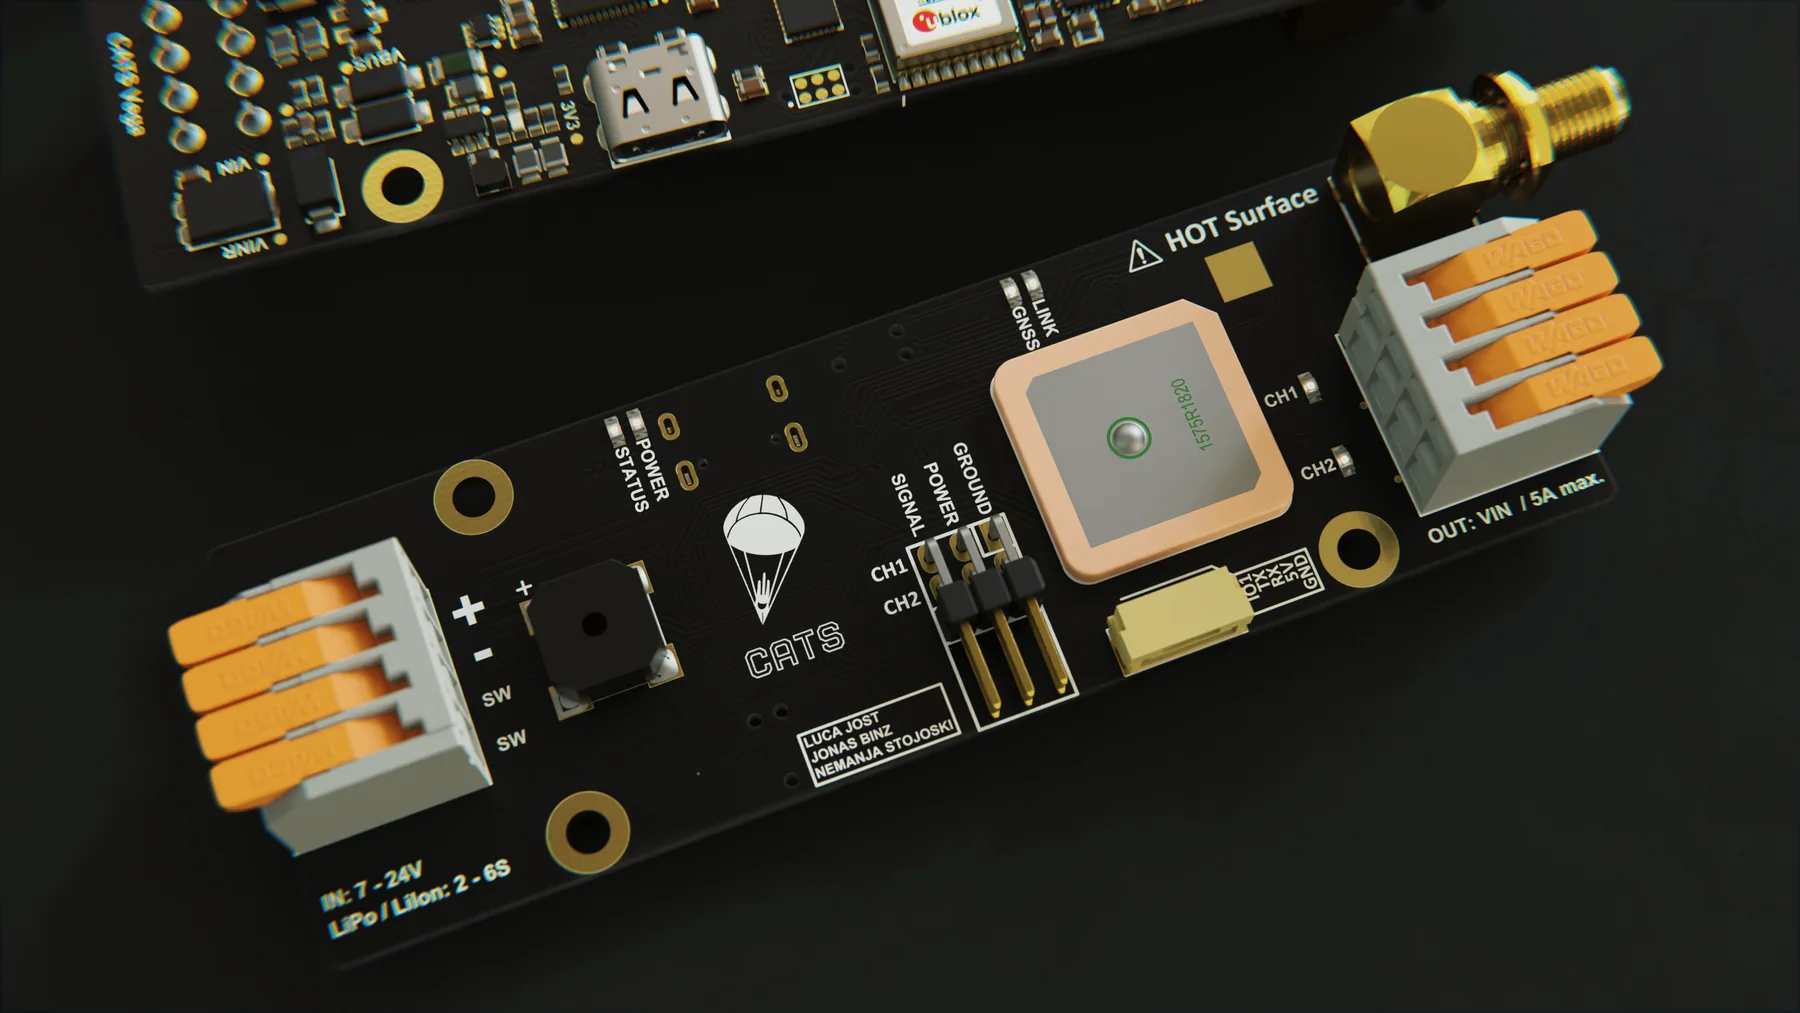
\includegraphics[width=\textwidth]{cats-vega}
        \caption{CATS Vega~\cite{cats:vega}.}
        \label{fig:cats-vega}
    \end{subfigure}
    \hfill
    \begin{subfigure}[b]{0.48\textwidth}
        \centering
        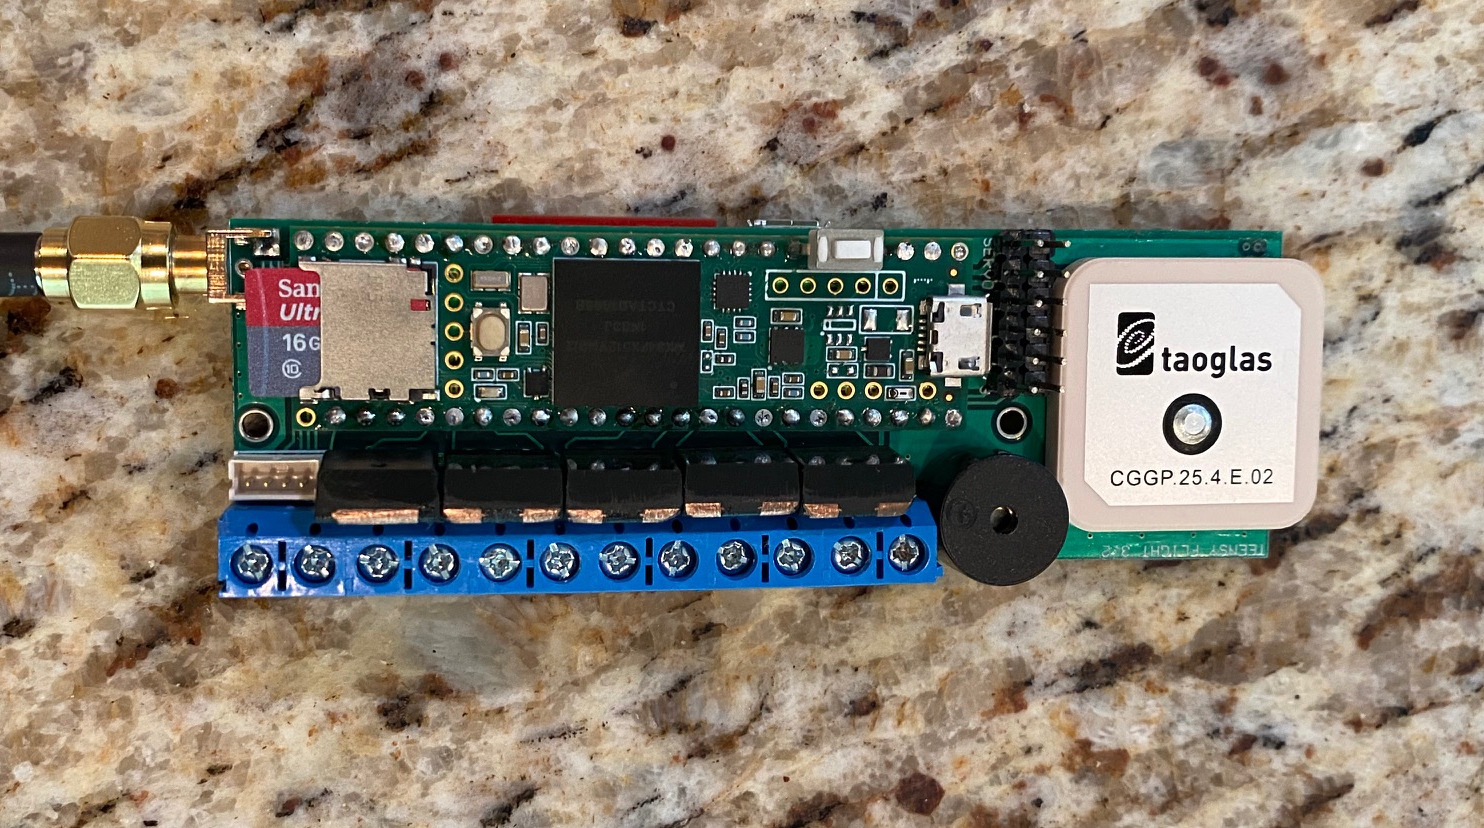
\includegraphics[width=\textwidth]{sparkyvt}
        \caption{HPR Rocket Flight Computer~\cite{sparkyvt:hpr-repo}.}
        \label{fig:sparkyvt}
    \end{subfigure}
    \caption{Open-source flight computers.}
    \label{fig:open-source-flight-computers}
\end{figure}


\paragraph{TUDSaT Zenith.} The Zenith is a flight computer developed by the RAPID student team of the Technical University of Darmstadt (TUDSaT) for their high-power hybrid rocket, which is expected to reach an apogee of $\SI{3}{km}$ at the EuRoC 2026 competition~\cite{tudsat:rapid}. % TODO: EuRoC 2026 takes place in October 2026. Verify the apogee after the competition 
The project is under active development, and the information reported here refers to the state of the repository at the time of writing~\cite{tudsat:zenithrepo}.

The board is based on an STM32H743 microcontroller and integrates redundant sensors: three barometric pressure sensors (MS5607, BMP580 and LPS22HB), three 6-axis IMUs (ICM-42670-P, ICM-42688-P and LSM6DSO32), a high-g accelerometer (H3LIS331DL), a magnetometer (LIS3MDL), a u-blox GNSS receiver, a W25Q SPI flash memory and a \SI{868}{MHz} LoRa transceiver~\cite{tudsat:zenithrepo}.

The firmware is written in Rust and uses the Embassy framework for embedded systems. A finite state machine (FSM) manages the flight phases, and the state of the rocket is estimated by combining two filters: a Mahony filter for the orientation and a 9-dimensional linear Kalman filter for the position, velocity and acceleration~\cite{tudsat:zenithrepo}.
The estimation runs at a frequency of \SI{1000}{Hz}~\cite{tudsat:zenithrepo}.

\paragraph{HPR Rocket Flight Computer.} The HPR Rocket Flight Computer is an open-source flight computer developed by an individual hobbyist, SparkyVT, for high-power rocketry~\cite{sparkyvt:hpr-repo}.

The board can be customised by the user: it is compatible with different microcontrollers of the Teensy family and can integrate different kinds of sensors. The default configuration includes a Teensy 4.1 microcontroller, an MS5611 barometric pressure sensors, an LSM6DSOX 6-axis IMU, an H3LIS331DL high-g accelerometer, a u-blox NEO-M9N GNSS receiver and an RFM96W or RFM95W LoRa transceiver, which can operate, respectively, in the \SI{433}{MHz} and \SI{868}{MHz} bands. The board can drive four pyrotechnic channels and eight servo channels.

The firmware is written in C++ using the Arduino framework. The altitude and the vertical velocity are estimated with a complementary filter that fuses barometric and inertial measurements at a frequency of ì\SI{1000}{Hz}. 
The orientation of the rocket is estimated by integrating the angular rate measured by the gyroscope according to the quaternion kinematics equations at a frequency of \SI{100}{Hz}.
The telemetry module transmits the GNSS position and the estimated state at a frequency of \SI{20}{Hz}, and the data can be visualised in real time on the ground station~\cite{sparkyvt:hpr-repo}. 

\paragraph{Vector II.} The Vector II is a sounding rocket developed by the State University of Londrina (UEL), Brazil, for educational and research purposes~\cite{NETZEL2026e00803}.

Its flight computer is based on an STM32F407 microcontroller and integrates an MS5607 barometric pressure sensor, an ICM-42670-P 6-axis IMU, an ADXL375 high-g accelerometer, an MMC5983MA magnetometer and a \SI{64}{Mbit} flash memory. It drives two pyrotechnic channels for the recovery system, which are fired once the apogee is detected.

The firmware uses the STMicroelectronics HAL library and implements a finite state machine (FSM) to manage the flight phases. The raw sensor measurements are stored in the flash memory at a frequency of \SI{12.5}{Hz}. The apogee is detected when the barometric pressure starts to increase monotonically~\cite{NETZEL2026e00803}. The system does not include a radio link and relies on post-flight analysis of the logged data.

% \begin{table}[htbp]
%     \centering
%     \small
%     \setlength{\tabcolsep}{4pt}
%     \caption{Estimation and telemetry capabilities of the open-source and student projects reviewed in this chapter.}
%     \label{tab:open-source-comparison}
%     \resizebox{\textwidth}{!}{%
%     \begin{tabular}{lcccc}
%         \toprule
%         \textbf{Project} & \textbf{MCU} & \textbf{Orientation est.} & \textbf{Position/velocity est.} & \textbf{Telemetry} \\
%         \midrule
%         CATS Vega & STM32F411 & Gyro integration & Vertical Kalman filter & LoRa, $\SI{2.4}{GHz}$ \\
%         TUDSaT Zenith & STM32H743 & Mahony filter & 9-state Kalman filter & LoRa, $\SI{868}{MHz}$ \\
%         HPR & Teensy 4.1 & Gyro integration & Complementary filter (vertical) & LoRa, 433/\SI{868}{MHz} \\
%         Vector II & STM32F407 & \cross & \cross & \cross \\
%         \bottomrule
%     \end{tabular}}
% \end{table}

\subsection{Summary and Open Issues}

Overall, the solutions reviewed in this section fall into two groups. Commercial flight computers are mature and well documented, and they are designed primarily around recovery and flight logging: barometric altitude and, in some models, inertial measurements are used to detect flight events, while GNSS receivers and telemetry are available only on the more complete devices. In the documentation reviewed, none of them provides an estimate of the full state of the rocket, and, with the exception of the Altus Metrum products, their hardware and firmware are not open. 

Open-source and student projects are more diverse. The CATS Vega and the TUDSaT Zenith combine onboard state estimation with a LoRa downlink, whereas the HPR Rocket Flight Computer estimates only the vertical channel and the Vector II logs the raw measurements without estimating the state or transmitting it. Among the projects considered, the orientation is obtained in most cases by integrating the angular rate of the gyroscope, which does not correct the drift of the estimate, and only the Zenith applies a dedicated attitude filter. Moreover, the design choices and the estimation algorithms are mostly documented in repositories and team websites rather than in peer-reviewed publications, which makes it difficult to compare them or to reproduce them.

To the best of our knowledge, no solution among those reviewed combines all of the following: a complete estimate of attitude, position and velocity based on sensor fusion, a telemetry link in a licence-exempt band suitable for European regulations, and a design simple and documented enough to be reproduced by a small team. This is the space addressed by this work, whose design choices are motivated in the next section.
